%%%%%%%%%%%%%%%%%%%%%%%%%%%%%%%%%%%%%%%%%%%%%%%%%%%%%%%%%%%%%%%%%%%%%%%%%%%%%%%%%%%%%%%%%%%%%%%%%
%
% Document:      DM  product tree
%
%%%%%%%%%%%%%%%%%%%%%%%%%%%%%%%%%%%%%%%%%%%%%%%%%%%%%%%%%%%%%%%%%%%%%%%%%%%%%%
\documentclass{article}
\usepackage{times,layouts}
\usepackage{tikz,hyperref,amsmath}
\usetikzlibrary{positioning,arrows,shapes,decorations.shapes,shapes.arrows}
\usetikzlibrary{backgrounds,calc}
\usepackage[paperwidth=55.8cm,paperheight=4.088cm,
left=-2mm,top=3mm,bottom=0mm,right=0mm,
noheadfoot,marginparwidth=0pt,includemp=false,
textwidth=30cm,textheight=50mm]{geometry}
\newcommand\showpage{%
\setlayoutscale{0.5}\setlabelfont{\tiny}\printheadingsfalse\printparametersfalse
\currentpage\pagedesign}
\hypersetup{pdftitle={DM products }, pdfsubject={Diagram illustrating the
products in LSST DM }, pdfauthor={ William O'Mullane}}
\tikzstyle{tbox}=[rectangle,text centered, text width=30mm]
\tikzstyle{wbbox}=[rectangle, rounded corners=3pt, draw=black, top color=blue!50!white, bottom color=white, very thick, minimum height=12mm, inner sep=2pt, text centered, text width=30mm]
\tikzstyle{pbox}=[rectangle, rounded corners=3pt, draw=black, top color=yellow!50!white, bottom color=white, very thick, minimum height=35pt, inner sep=2pt, text centered, text width=35mm]
\tikzstyle{pline}=[-, thick]
\begin{document}
\begin{tikzpicture}[node distance=0mm]
\node (DAC) [pbox, 
] {\textbf{Data Access Center} };
\node [below right] at (DAC.north west) {\small \color{blue}.} ;
\node (DBB) [pbox, 
right=6.2cm of DAC] {\textbf{Data Backbone} };
\node [below right] at (DBB.north west) {\small \color{blue}.} ;
\node (DEVEL) [pbox, 
right=6.2cm of DBB] {\textbf{Developer services} };
\node [below right] at (DEVEL.north west) {\small \color{blue}.} ;
\node (IDM) [pbox, 
right=6.2cm of DEVEL] {\textbf{Identity Manager} };
\node (INFRA) [pbox, 
right=6.2cm of IDM] {\textbf{Infrastructure} };
\node [below right] at (INFRA.north west) {\small \color{blue}.} ;
\node (INTGTEST) [pbox, 
right=6.2cm of INFRA] {\textbf{Integration Test} };
\node [below right] at (INTGTEST.north west) {\small \color{blue}.} ;
\node (ITENV) [pbox, 
right=6.2cm of INTGTEST] {\textbf{IT Environments} };
\node [below right] at (ITENV.north west) {\small \color{blue}.} ;
\node (L1) [pbox, 
right=6.2cm of ITENV] {\textbf{Level 1 System} };
\node [below right] at (L1.north west) {\small \color{blue}1.02C.03} ;
\node (L2) [pbox, 
right=6.2cm of L1] {\textbf{Level 2 System} };
\node [below right] at (L2.north west) {\small \color{blue}.} ;
\node (LSP) [pbox, 
right=6.2cm of L2] {\textbf{Science Platform} };
\node [below right] at (LSP.north west) {\small \color{blue}.} ;
\node (NETDM) [pbox, 
right=6.2cm of LSP] {\textbf{DM Networks} };
\node [below right] at (NETDM.north west) {\small \color{blue}.} ;
\node (SCIALG) [pbox, 
right=6.2cm of NETDM] {\textbf{Science Algorithms} };
\node [below right] at (SCIALG.north west) {\small \color{blue}.} ;
\node (SCIPRIM) [pbox, 
right=6.2cm of SCIALG] {\textbf{Science Primitives} };
\node [below right] at (SCIPRIM.north west) {\small \color{blue}.} ;
\node (SQUASH) [pbox, 
right=6.2cm of SCIPRIM] {\textbf{QC Dashboard} };
\node [below right] at (SQUASH.north west) {\small \color{blue}.} ;
\node (DM) [wbbox, above=15mm of L1]{\textbf{Data Management}};
 \draw[pline]   (DAC.north) -- ++(0.0,0.5) -| (DM.south) ; 
 \draw[pline]   (DBB.north) -- ++(0.0,0.5) -| (DM.south) ; 
 \draw[pline]   (DEVEL.north) -- ++(0.0,0.5) -| (DM.south) ; 
 \draw[pline]   (IDM.north) -- ++(0.0,0.5) -| (DM.south) ; 
 \draw[pline]   (INFRA.north) -- ++(0.0,0.5) -| (DM.south) ; 
 \draw[pline]   (INTGTEST.north) -- ++(0.0,0.5) -| (DM.south) ; 
 \draw[pline]   (ITENV.north) -- ++(0.0,0.5) -| (DM.south) ; 
 \draw[pline]   (L1.north) -- ++(0.0,0.5) -| (DM.south) ; 
 \draw[pline]   (L2.north) -- ++(0.0,0.5) -| (DM.south) ; 
 \draw[pline]   (LSP.north) -- ++(0.0,0.5) -| (DM.south) ; 
 \draw[pline]   (NETDM.north) -- ++(0.0,0.5) -| (DM.south) ; 
 \draw[pline]   (SCIALG.north) -- ++(0.0,0.5) -| (DM.south) ; 
 \draw[pline]   (SCIPRIM.north) -- ++(0.0,0.5) -| (DM.south) ; 
 \draw[pline]   (SQUASH.north) -- ++(0.0,0.5) -| (DM.south) ; 
\end{tikzpicture}
\end{document}
